\chapter[SCP-100 Jamaican Joe的废品嘉年华]{
    SCP-100 "Jamaican Joe's Junkyard Jubilee"\\
    SCP-100 Jamaican Joe的废品嘉年华
}

\label{chap:SCP-100}

\begin{figure}[H]
    \centering
    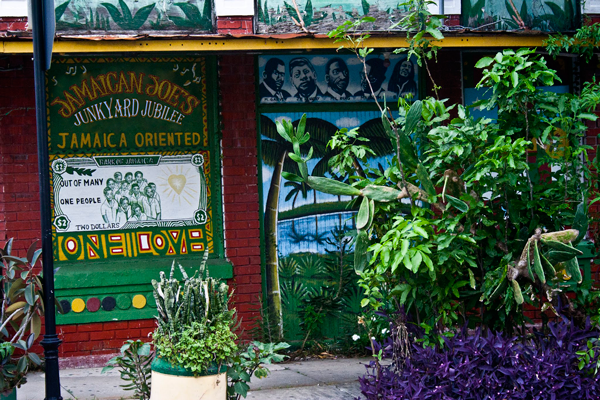
\includegraphics[width=0.5\linewidth]{images/SCP.100.png}
    \caption*{SCP-100的店面,外观}
\end{figure}

\bb{项目编号:}SCP-100

\bb{项目等级:}Euclid

\bb{特殊收容措施:}SCP-100的栅栏区域内有6名守卫进行巡逻,还有2名守卫负责监控内部和外部的仓库和住宅建筑,每3小时轮换一次。在SCP-100内发现任何未经授权的人员将被扣留和讯问,随后实行记忆消除并释放。

3名守卫,将留在SCP-100的店面内,每8小时轮换一次。店面正门应随时保持锁住,只有必要人员才持有钥匙。“私人财产”和“不得翻越”的警告标志应放置在店面前,以阻止任何司机停在SCP-100停留。

任何被SCP-100-1所制造的物品将被移出SCP-100并溶解成渣,除了SCP-100-2-A和SCP-100-2-B例外。若任何SCP-100-1变得不合作,SCP-100-2-A和SCP-100-2-B将被移出SCP-100直到SCP-100-1变得再次合作为止。

SCP-100内最大的两个仓库将被改装成基础研究设施。所有由SCP-100-1制造的物品,包括SCP-100-2-A和SCP-100-2-B,都可以用于研究目的。对SCP-100-1本身的测试则需要首席研究员的书面批准。

\bb{描述:}SCP-100是位于南卡罗莱纳州的一个废弃的废品堆放站,离█████████有80公里,最为知名的名字是“Jamaican Joe's Junkyard Jubilee”。该堆放站拥有5000平方米用栅栏围起的土地,包括两个仓库,一个店面,和一个小型的居住建筑,包括空地(neglected land,原意为被忽略的土地)和用于储存的面积。SCP-100收容有约1500辆汽车,包括已经被压扁和还没处理的,还有约1400公斤的零碎金属,价值约5000美元(3870欧元)。

SCP-100的异常效应体现在SCP-100-1和其造物上,包括SCP-100-2-A和SCP-100-2-B。项目会在SCP-100-1或其造物穿过SCP-100的栅栏时失去自主可动性,并保持该状态直到上述个体归还为止。

SCP-100-1是一个有自我意识的,有感知的,人形造物,由一系列钢管,未绝缘的铜线,和铝罐组成。SCP-100-1缺少进行书面或口头沟通的能力,尽管如此它有能力通过基本的信号(灯光)语言进行交流。SCP-100-1很大部分程度上不太关心外部销售和它被限制起来的信息。SCP-100-1似乎展示出制造技巧,并证明有能力操作诸如电焊机,钻头,和电锯,以及重型机械诸如车辆压缩机和铲车。

SCP-100-1展示出可以制造和其异常特性类似的个体,通过使用SCP-100内的各种材料,SCP-100-1创造了4个特殊动物-鬣蜥,鳄鱼,乌龟,和火烈鸟-尽管如此,SCP-100-1已知还创造过其他物种,诸如宠物。为了保持其顺从,SCP-100被允许持有2个物品,标记为SCP-100-2-A和SCP-100-20-B。

\begin{figure}[H]
    \centering
    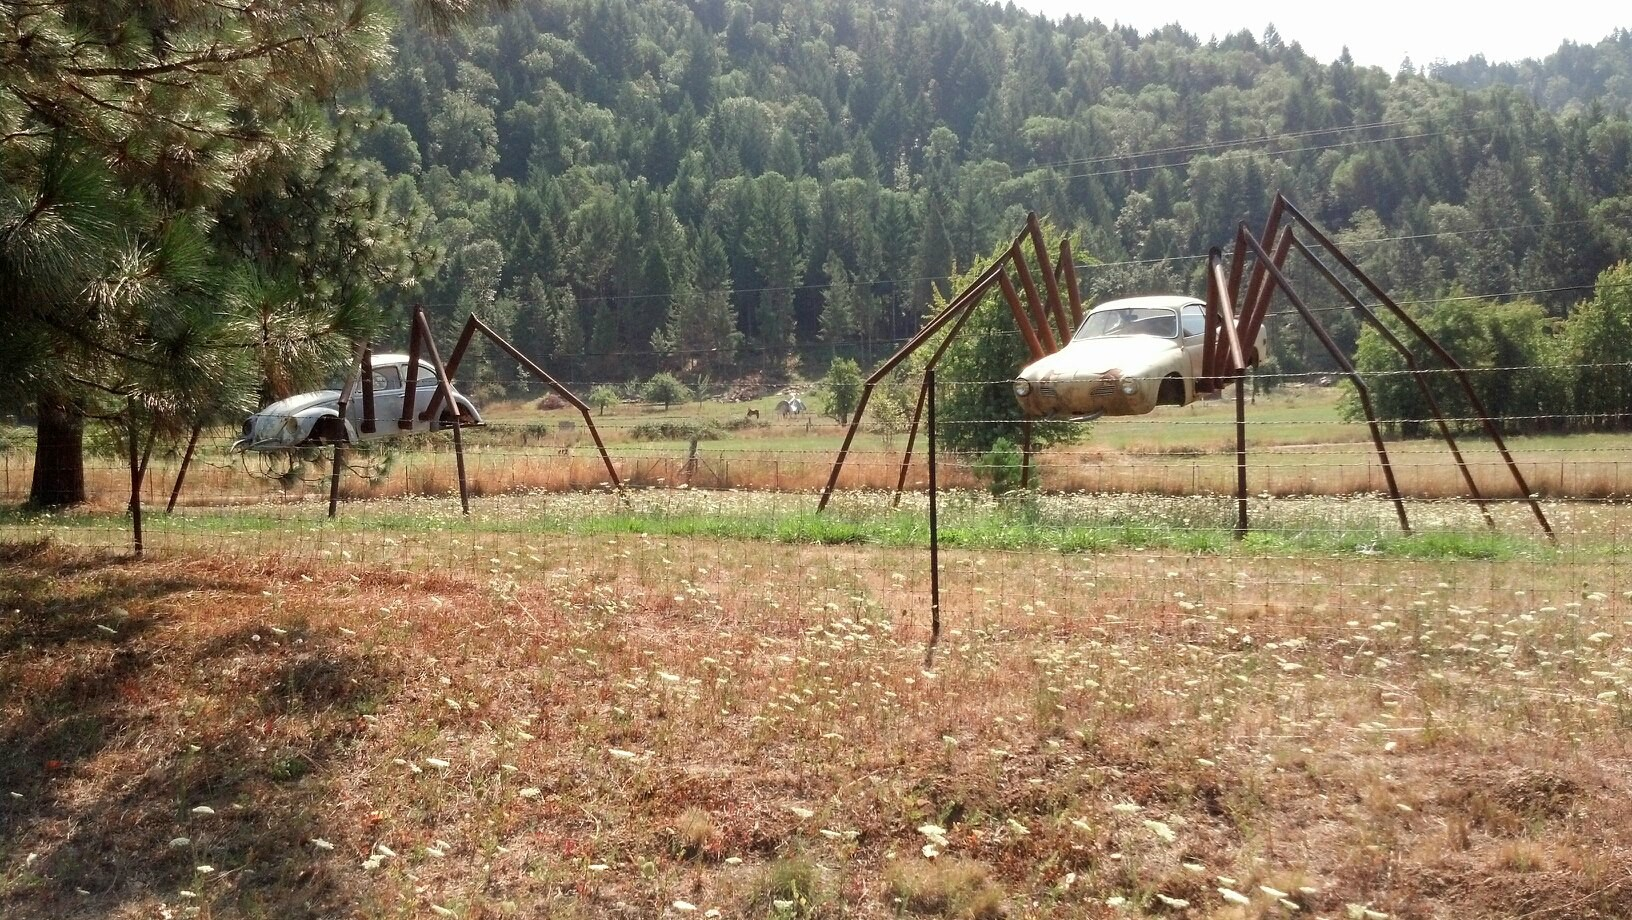
\includegraphics[width=0.5\linewidth]{images/SCP.100.2.jpg}
    \caption*{SCP-100-2-A和SCP-100-2-B正巡逻临时围栏的维修}
\end{figure}

SCP-100-2-A和SCP-100-2-B设计表面上类似于昆虫,假定是由SCP-100制造,因为它们在初次发现SCP-100时就占据了此处。SCP-100-2-A和SCP-100-2-B的背后分别印有名字“Raymone”和“Beatrice”。它们似乎同时作为同伴运作并守卫SCP-100,它们只在与SCP-100-1交流的间隔才停下,其他时间都在SCP-100的范围内巡逻。

SCP-100-1似乎服从一种仪式安排,每日重复以下行为。

\begin{itemize}
\item 在0800时到1500时,SCP-100-1进入SCP-100的店面,坐在柜台后面并试图和进入店面的人类谈价。偶尔的,SCP-100-1会较早的回到堆放场内,理由未知。
\item 在1500时到1600时,SCP-100-1通过模糊手势和脚步运动进行和SCP-100-2-A和SCP-100-2-B进行交流。交流内容包括装饰,修理,以及类似“取物”和“捉迷藏”的行为。
\item 在1600时到2000时,SCP-100-1进行各种工作,包括从SCP-100内取得材料,清扫和维护工具以及重型机械,并清扫SCP-100内建筑物的内部和外部。
\item 在2000时到0000时,SCP-100-1进行假定为休闲的行为,行为包括制造新物品,和SCP-100-2-A和SCP-100-2-B交流,在SCP-100内巡逻等。
\item 在0000时到0080时,SCP-100-1进入住宅建筑,并在此期间一直坐在书桌后面。
\end{itemize}

若在SCP-100-1坐在柜台后时有人类进入SCP-100的店面,SCP-100-1将试图与他们交易,使用各种手势来表达意思。SCP-100-1大部分情况试图出售废品,它自己的造物,或修理服务,尽管如此它知道如何购买废品。尽管SCP-100-1无法阅读,但是它在销售中显示出有基础的数学计算能力。

SCP-100-1所做的销售显示出某种程度的不公平。SCP-100-1会故意出售用便宜金属制作的有缺陷的天平和有污渍的废品堆,并似乎有关于SCP-100效应的知识,因为SCP-100-1不停重复出卖造物,尽管其自主移动性在离开SCP-100后就消失了。遭遇SCP-100-1将会面对窘迫和冷漠,其墙上贴着标语“不退货,伙计!”,无论SCP-100-1的情绪反应如何。

SCP-100发现于11\slash 09\slash 76,当时有报告有奇怪的机械在废品堆放场内活动。这些流言被视为都市传说,而基金会派了一名特工去SCP-100去冒充土地所有者,直到收容通过不动产购买完成。一道木质栅栏沿着之前SCP-100的栅栏建立起来,在店面里装上了单面窗户(从外面无法看见里面),而一条穿越附近█████████镇的高速公路使得大部分公众交通改道。

\bb{附录100-A:}记录显示此处拥有者为“Joseph Duval”,其邮政地址也使用同样的名字。当地账务公司报告其账单在SCP-100发现的3个月前停止了,只留下SCP-100-1,SCP-100-2-A,SCP-100-2-B,以及数只假定被SCP-100-1创造的鸟类和犬类个体。对建筑物的初次扫除发现住宅建筑的大部分都空空如也,唯一显示前主任的信息是一张写在纸条上挂在店面门上的纸条。(见\bb{文件100-A})

\bb{事故100-A:}在06\slash 03\slash 05,SCP-100-1创造了一个有自我意识,10厘米高的人形,这是SCP-100-1第一次创造人形。其在该造物上用了比其他造物更多的努力,该造物上拥有极其精细的细节,包括面部特征,和印在造物背后的“J.J.”字样,造物的大部分都是由不锈钢制成。SCP-100-1在时间表间隔期间将造物放置在店面的柜台上,并互相使用各种手势进行明显的交流。在和造物进行交流之后,SCP-100-1在SCP-100内的住宅建筑内坐了将近10天。

\bb{文件100-A:}下列是在SCP-100内回收的备忘的一份拷贝。

\begin{scpbox}
\centering
出去吃午饭,请找助手-J.J.
\end{scpbox}
